\section{Задача 2.13}
\subsection{Задание:}
Составить квадратное уравнение с целыми коэффицентами и отрицательным дискриминантом и решить его.
\subsection{Решение:}
Решим уравнение $ x^2 + 2x + 2 = 0 $.
\\
$
	D = 4 - 4 \cdot 1 \cdot 2 = -4
	\\[1em]
	x = \dfrac{-2 \pm \sqrt{-4}}{2}
	\\[1em]
	x = \dfrac{-2 \pm 2i}{2} = -1 \pm i
$
\subsection{Компьютерная проверка в среде Wolfram Mathematica:}
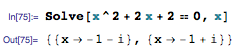
\includegraphics[scale=0.6]{task/2_13/screen.png}
